

\documentclass[12pt]{article}
\usepackage[T1]{fontenc}
\usepackage[utf8]{inputenc}
\usepackage{amsmath}
\usepackage{microtype}
\usepackage{listings}
\setlength{\parindent}{0pt}
\usepackage{fancyvrb}
\usepackage{enumerate}
\usepackage{array}
\usepackage[breaklinks=true,linktocpage,hidelinks]{hyperref}
\usepackage[letterpaper]{geometry}
\usepackage{url}
\usepackage{graphicx}
\usepackage{fullpage}
\usepackage{caption}
\captionsetup{labelfont={bf,small,sf}, textfont={small, sf}}
\usepackage[sc]{mathpazo}

\usepackage{pgfplots}
\usepackage{pgfplotstable}
\usepackage{tikz}

\usepackage{fancyhdr}
\usepackage{fancybox}
\usepackage{multicol}
\usepackage{xcolor}
\usepackage{adjustbox}
\usepackage{wrapfig}



\pgfplotsset{compat=newest}
\usetikzlibrary{shapes,backgrounds,arrows}
\usepgfplotslibrary{external} 

\definecolor{brewcol1}{RGB}{166,206,227}
\definecolor{brewcol2}{RGB}{31,120,180}
\definecolor{brewcol3}{RGB}{178,223,138}
\definecolor{brewcol4}{RGB}{51,160,44}
\definecolor{brewcol5}{RGB}{251,154,153}
\definecolor{brewcol6}{RGB}{227,26,28}
\definecolor{brewcol7}{RGB}{237,179,1}
\definecolor{brewcol8}{RGB}{202,178,214}
\definecolor{brewcol9}{RGB}{206,27,1}

\definecolor{brewforest1}{RGB}{65,171,93}
\definecolor{brewforest2}{RGB}{161,217,155}
\definecolor{brewforest3}{RGB}{49,163,84}

\geometry{hmargin=1.87cm, vmargin=1.87cm}
\bibliographystyle{siam}

\DeclareTextFontCommand{\helvetica}{\fontfamily{phv}\selectfont\small}


\begin{document}

\clearpage\thispagestyle{empty}
\begin{center}
\textbf{Difficult transition for sugar maple in Boreal forest under climate change? \\
Impact of alternative stable states on Sugar maple migration.}
\vskip 2em
Research proposal
\vskip 1em
Master in Wildlife management
\vfill
By
\vfill
Steve Vissault 
\vfill 
For
\vfill
\textbf{Richard Cloutier}, Pr.\\
Director of the program committee
\vskip 2em
\textbf{Dominique Arsenault}, Pr.\\
President of the jury
\vskip 2em
\textbf{Matt Talluto}, PhD\\
Research Co-director
\vskip 2em
\textbf{Dominique Gravel}, Pr.\\
Research Director
\vfill
\vfill
Université du Québec à Rimouski\\
\today

\end{center}

\newpage
\setcounter{page}{1}

\section{Introduction}

The boreal region is warming twice as fast as the global
average and  this will inevitably alter the species composition in boreal
forests \cite{Scheffer2012,Hughes2000}. Sugar maple (\textit{Acer saccharum})
is a widespread and abundant tree in north-eastern North America and is one of
the most representative species of northern temperate forests
\cite{Graignic2013,Messaoud2007,Kellman2004,Barras1998}. This species is one
of the species expected to migrate northward towards the northern limit of the
temperate forest \cite{McKENNEY2007,Goldblum2005}. Predicting shifts in the
range of sugar maple under climate change is an important challenge because
this species is highly desirable by hardwood and maple syrup producers, two
large economic sectors in Quebec. This expected northward migration of sugar
maple and its vegetal community might increase the ecotone between the boreal
and temperate forest of Québec.\\

Some species mostly representative of northern forest ecosystems are predicted
to expand their distribution range broadly to the north. As an example, sugar
maple is expected to move northward closed to the Ungava bay
\cite{McKENNEY2007}. These predictions are built on species distribution models
based only on climatic conditions though maple regeneration depends both on
macroclimatic (\textit{i.e.} regional climate) and microclimatic conditions
(\textit{i.e.} soil conditions). Thus, the expansion of this species
distribution is difficult to predict because microconditions (\textit{e.g.}
soil moisture, pH) can mitigate macroconditions such as global warming
\cite{DeFrenne2013}. Even if the regional climate conditions are favorable
\cite{Kellman2004}, the microconditions found in the boreal forest could
affect the establishment of sugar maple
\cite{Kellman2004,Moore2008,DeFrenne2013,Barras1998}. For instance, in boreal
forest, colder temperatures from shading and excess soil moisture due to snow
melt cause litter to be more acidic and fibrous during the spring  when the
seeds are supposed to be germinating (\textbf{Source}). The maple could then
be unable to migrate in boreal forests as a result of negative local
feedbacks. Thus, the landscape structure could be seen as a patchy mosaic
structure where stand soil conditions are driving the spatial occurences of
boreal and temperate species stands despite a regional climate favorable to
temperate species. In this case, boreal and temperate stands are two
alternative stable states, \textit{i.e.} contrasted states occuring in the
same climate conditions. This situation generate a tension between the boreal
and temperate forest meaning that soil perturbations can produce drastic shift
in community composition in the boreal-temperate forest ecotone.

% DG: be careful to use constant terminology, avoid switch between terms, such as macroclimate and regional climate. Define all terms.


\section{Objectives.}


The main objective of this project is to investigate the transition dynamic
between the boreal and temperate forests under different climate change and
management scenarios. In this context, we will test four different hypothesis:
($H_1$) Alternative stable states are occuring in the boreal-temperate forests
ecotone; ($H_2$) Regional climatic conditions are not the main attractor of
alternative stable states in the boreal-temperate forest ecotone; ($H_3$)
Climate change will increase the frequency of alternative stable state
occurence; ($H_4$) Forest management is a main attractor of alternative stable
states, increasing the rate of transition towards temperate forest patches. In
order to test the hypothesis, I will (1) create a model of the transition
between temperate and the boreal forest; (2) investigate the spatial structure
and presence of alternative stable states in the transitional zone; and
finally (3) run simulations based on different climate change and management
scenarios.\\

This project's proposal contain a first section of review subdivided into two
parts. The first part presents the theoretical context on alternative stable
states and abrupt changes in ecosystems functioning. The second part of this
review focuses on transition in boreal-temperate forest system and explain why
alternative stable states is a relevant framework to study the dynamic of the
boreal-temperate forests ecotone.  The second section of this document
describes the model and the methodology employed to assess the objectives. To
conclude, the last part presents the general timeline associated with this
project.

%%% Question from hedvig: What is the relationship between the temperatre forest and the sugar maple?

\section{Review} 

\begin{figure}[t]
	\begin{center}
	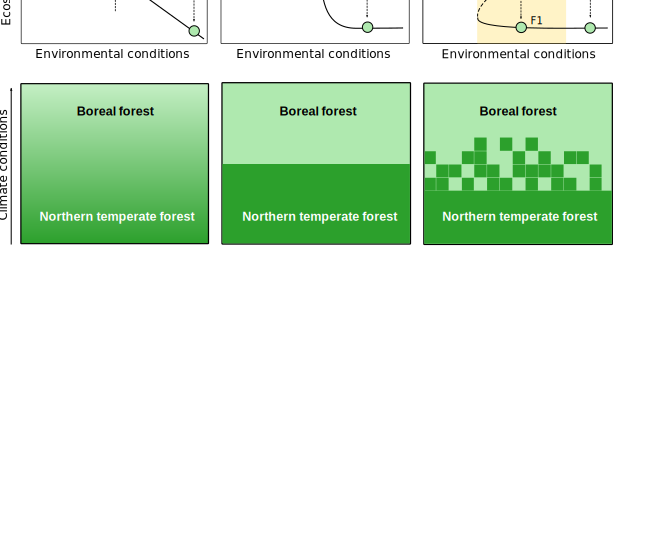
\includegraphics[width=0.8\textwidth]{fig/states.pdf}
	\end{center}
	\caption{Schematic representation of different ways in which the equilibrium
	states from forest-forest system can vary with conditions such as temperature, precipitation
	or soil moisture. Three differents kinds of respond are presented,
	\textbf{(A)} gradual, \textbf{(B)} basic fold, \textbf{(C}) catastrophic fold.
	The first panels line is a conceptualization of a transitional landscape
	between two forest ecosystems. The second panels 
	line presents the stable states rise by the forest
	given a specific environnemental condition. Each arrows in graphs indicate the
	point toward the system moves if it's not at the equilibrium. Every point on
	the plain line could be a stable state encounter by the boreal-temperate
	forests system, excepted for the dashed line (in yellow highlight). This zone,
	called hysteresis, are particulary unstable and little fluctuations in
	environnement conditions give rise to a contrasted state representing an
	alternative stable states. ($F_1$ or $F_2$).}
	\label{fig1}
\end{figure}


\textbf{Alternative stable state in forest ecosystems.}  Many ecotone studies
and modeling efforts focus on transition between forest to non-forests (e. g.
Boreal - Tundra) \cite{Scheffer2012,Scheffer2001,Hirota2011,Messaoud2007} but
little attention has been given to evaluate the transitional dynamics of
forest- forest ecotones \cite{Goldblum2010,Graignic2013}. At large scale,
transitions between  the temperate and boreal forests can be approached as a
dynamic system where each forest biome is a stable state. The presence of
different states at a location or a time depends on environmental conditions
(e. g. soil, temperature). When small environmental fluctuations occur, most
dynamical systems respond almost linearly with no threshold drastic changes in
the state of the ecosystem ( Figure \ref{fig1} .a)
\cite{Scheffer2001,Scheffer2009}. In this case, only one equilibrium can be
observed given a specific environmental condition
\cite{Scheffer2001,Scheffer2009,scheffer2009critical}. For instance, when the
soil moisture increase slowly the new condition obtained might cause favorable
conditions to a new species introduction but this  don't change the ecosystem
functionning. Another kind of response occurs more frequently in nature.
Natural systems are insensitive to environmental conditions over certain
ranges but respond strongly when a threshold is reached (Figure \ref{fig1} .b)
\cite{scheffer2009critical}. Tree mortality can increase sharply when a toxin
is added to the environment. \cite{scheffer2009critical}. In this case, the
response curve of the natural systeme is not linear but lightly folded and a
small change can drive the sytem to a treshold and lead to major changes.
Small changes in the initial conditions can transform abruptly the species
community composition and lead to a strong spatial division as representing in
figure \ref{fig1}.c (Upper panel). In an other hand, respond curve can be
folded backwards and the same threshold can conduct the system into
catastrophic changes (Figure \ref{fig1} .c).  When the system approach a
tipping point on the folded upper branch, the system cannot pass smootly to
the lower branch. Small forcing on initial condition of the state $F_1$
transfer immediatly the system into a contrasted state $F_2$ (Figure
\ref{fig1} .c). This point is called \textit{Bifurcation point} and small
forcing on those critical states can drive the system into backward or forward
shifts, increasing catastrophic events. In this situation, the system present
alternative stable states who mean the presence of contrasted states over
certain range of environmental conditions \cite{scheffer2009critical}. This
range can be spatially structured as an intermixed of constrasted patches in a
ecotone landscape like shown across the sub-figure \ref{fig1} .c (upper part).
This layout could be easily rattached to the hardwood-boreal forest patchiness
structure often attribute to differences in soils, nutrient status and
topographical factors \cite{Society2014}.\\

\textbf{Natural system.} In the boreal-temperate forest ecotone, there is no
distinct boundary and a broad transition zone exists composed of mixed stands
of coniferous-deciduous species \cite{Goldblum2010}. Instead a macromosaic
landscape can be observed with pure stands of deciduous trees on favorable
sites and pure coniferous stands on less favorable sites \cite{Goldblum2010}.
This segregated patches distribution could be explain by the fact than
microclimatic conditions can modulate establishement of those forests
\cite{DeFrenne2013}. Distribution of deciduous and boreal forests within
ecotone is not determined only along environnemental gradients present on
large scales but rather by local variation and conditions in substrate,
drainage, physical soil properties, and nutrient avaiblity
\cite{Goldblum2010,Society2014}.  By example, balsam fir (\textit{Abies
balsamea}) is often related to thick organic horizons and coarse xeric
deposits while sugar maple is mostly present in opposite edaphic conditions
\cite{Messaoud2007,Kellman2004,Barras1998}. Moreover, boreal and hardwood
forests are dominated by trees of distinctive physiognomy which may be
expected to produce distinctive litter and light micro-environments
\cite{Barras1998}. Those dominant species might induce conditions that
differentially facilitate regeneration of the community’s species as positive
feeback which contribute to preserve the community type \cite{Barras1998}.
Frelich \textit{et al.}(1993) \cite{Society2014} hypothesized sugar maple has
one of those species.  Knowing this, the alternative stable states is a
relevant framework to study this ecotone dynamic because the soil conditions
and role of dominant species in regeneration seems to act as main feedbacks on
the temperate forest establishment generating a patchiness landscape (Figure
\ref{fig1}.c, upper panel). In this context, we expected to find patch
dominated by boreal species and others dominated by temperate species under a
certain range of climatic conditions. Thus, the soil condition and the role of
dominant species in boreal and temperate forest need to be investigate as main
drivers in alternative stable states
\cite{Kellman2004,Moore2008,DeFrenne2013,Barras1998}.


% We used maple sugar basa areal in function of black
% spruce, white spruce and balsam fir basal area to compute the relative
% abundance of sugar maple. Given the above statements, we used mainly two
% climatic variables (annual mean temperature and annual precipitation) to
% identify the alternative stable states present in the boreal-temperate
% ecotone. The relationship was performed on climatic variables and sugar maple
% relative abundance using kernel density plot function. We obtained the
% probability of observed a sample plot as function of sugar maple relative
% abundance and mean annual temperature (Figure \ref{fig1}). In both case,
% alternative stable states are presents whereas the function graphed has a
% bimodal distribution. At low precipitation or temperature conditions, the
% probability of observing a parcel sampled without sugar maple is higher than
% intermediate climatic conditions where the multimodal distribution appear. The
% density function suggest the presence of alternative stabe states  in response
% of intermediate climatic conditions: one state wherein sugar maple dominates
% and an another in which sugar maple is absent. \\

\section{Methods}   

\begin{wrapfigure}{L}{0.45\textwidth}         
	
	\begin{figure}[!ht]
\begin{center}
	
				\tikzstyle{noeud}=[circle,
				                  thick,
				                  minimum size = 1.5cm,
				                  inner sep =5pt,
				                  draw=brewforest3,
				                  fill=brewforest1]
				\tikzstyle{noeud2}=[circle,
				                  thick,
				                  minimum size = 1.5cm,
				                  inner sep =5pt,
				                  draw=brewforest3,
				                  fill=brewforest2]
				\tikzstyle{noeud3}=[circle,
				                  thick,
				                  minimum size = 1.5cm,
				                  inner sep =5pt,
				                  draw=brewforest3,
				                  fill=brewforest3]
	
				\begin{tikzpicture}[->,>=stealth',auto,scale=0.8]
				      \node [circle,noeud2] (M) at (0,0) {\textbf{M}};
				      \node [circle,noeud2]  (C) at (-5,5) {\textbf{C}};
				      \node [circle,noeud2] (D) at (5,5) {\textbf{D}};
				      \node [circle,noeud2] (T) at (0,10) {\textbf{T}};
	
						\draw[thick,-latex] (M) to[bend right=10] node[above,sloped] {$S_C$} (C);
						\draw[thick,-latex] (C) to[bend right=10] node[below,sloped] {$\beta_d \cdot (C+M)$} (M);
	
						\draw[thick,-latex] (D) to[bend right=10] node[above,sloped] {$\beta_c \cdot (D+M)$} (M);
						\draw[thick,-latex] (M) to[bend right=10] node[below,sloped] {$S_D$} (D);
	
						\draw[thick,-latex] (D) to[bend right=10] node[above,sloped] {$e$} (T);
						\draw[thick,-latex] (T) to[bend right=10] node[below,sloped] {$P_D$} (D);
	
						\draw[thick,-latex] (T) to[bend right=10] node[above,sloped] {$P_C$} (C);
						\draw[thick,-latex] (C) to[bend right=10] node[below,sloped] {$e$} (T);
	
						\draw[thick,-latex,transform canvas={xshift=0.8ex}] (T) to node[above,sloped,rotate=90,transform canvas={xshift=5ex}] {$P_D \cdot P_C$} (M);
						\draw[thick,-latex,transform canvas={xshift=-0.8ex}] (M) to node[above,sloped,rotate=-90,transform canvas={xshift=-3ex}] {$e$} (T);
				\end{tikzpicture}
	
			\caption{Conceptual transition model between forest stands deciduous ($D$), mixte ($M$) and coniferious ($C$). $E$ corresponds to a transitionnal state where a perturbation are occurred with a frequence of $e$. Parameters $\beta$ and $S$ are referred as the colonisation and the succession rates respectively. We defined the recovery rates ($P_C$ et $P_D$) as $P_C = \alpha_C \cdot (M+C) \cdot [1- \alpha_D \cdot (D +M)]$ and $P_D = \alpha_D \cdot (D+M) \cdot [1- \alpha_C \cdot (C +M)]$, to finaly get this equation $P_M = P_C \cdot P_D$. The parameter $\alpha$ mean the recovery rate after a patch has been disturbe.}

	\end{center}	
	\label{Model}
\end{figure}
	\caption{Conceptual transition model between forest stands deciduous ($D$),
	mixte ($M$) and coniferous ($C$). $T$ corresponds to a transitionnal state
	where a perturbation are occurred with a frequence of $e$. Parameters $\beta$
	and $S$ are referred as the colonisation and the succession rates
	respectively. We defined the recovery rates ($\phi_c$ et $\phi_d$) as $\phi_c
	= \alpha_c \cdot (M+C) \cdot [1- \alpha_d \cdot (D +M)]$ and $\phi_D =
	\alpha_d \cdot (D+M) \cdot [1- \alpha_c \cdot (C +M)]$, to finaly get this
	equation $\phi_m = \phi_c \cdot \phi_d$. The parameter $\alpha$ mean the
	recovery rate after a patch has been disturbe.}         
	\label{Model}
\end{wrapfigure}


Following this review, the first methodology section will describe the general
model reproducing the boreal-temperate ecotone dynamic. The second part will
be adressed on data used on the parametrization and calibration of this model.
Whereas the transition between temperate and boreal forests is influenced by
environnemental conditions and proportion of coniferious and deciduous
available in the neighbourhood, the third section section will dedicated on
those factors and their parametrization. Two last sections will focus on
simulation and validation techniques used in this project's context.\\

\textbf{Models.} This state and transition model will be based on three
different forest states: \textbf{(D)} Deciduous and \textbf{(M)} Mixed patches
characterizing temperate forests, then \textbf{(C)} Coniferous patch
representing boreal forests (Figure \ref{Model}). Disturbances regime is a
main driver in those forest dynamics (e .g. Fire in boreal forest or frost in
temperate forest). When gap event occur in deciduous patch, species presents
will be replaced by shade intolerant species as aspen and white birch, well
adapted to the new shading condition. Thus post-disturbance patches has been
integrated within the model across the transitional patch \textbf{(T)} (Figure
\ref{Model}).  On long term, late-succesional species from the understory will
take up giving a new state (C, D or M). All states can change to another state
except the direct transition between a deciduous and coniferous stands which
doesn't occur in natural systems. Simulations of this model aims to assess the
transition rate between each state in the overall landscape and identify if
deciduous and coniferous patches are present as alternative stable states.
When a coniferous patch $C$ has been disturbed with a rate $e$, this can be
recovered to another state following $\phi_c$. This term is taking in account
a specific patch recovery rate ($\alpha_{c}$), the availability of coniferous
species ($M+C$) and the proportion of paths unconverted into a deciduous state
($1- \alpha_d \cdot (D +M)$). In making the assumption that perturbation rate
is similar between states, dynamic of a patch $T$ can be formally describe by
these differential equations: $\frac{\delta T}{\delta t} = e \cdot (C+M+D) - T
\cdot (\phi_d + \phi_c + \phi_m)$. If a patch $C$ is undisturbed, deciduous
species $(D+M)$ can spread over the patch with a colonisation rate $\beta_d$
giving a new mixed patch. A mixed stand $M$ might turn into a coniferous stand
with a sucession rate $S_c$.  We can also summarize the coniferous dynamic by
this differential equation: $\frac{\delta C}{\delta t} = \phi_C \cdot T + S_c
\cdot M - \alpha_d \cdot (D+M)\cdot C - e \cdot C$. At this stage of this
project, the model is spatially implicit and assume that all space is occupied
by one state, so that the proportions of land cover occupied by all types of
patch sum to 1. The model will be solved numericaly and discretize (\textbf{Note:} Not
sure to be enough comfortable to discuss about the last sentence).\\

\textbf{Data description.}  The parameterization and validation of this model
will be conducted on the QUICC-FOR\footnote{Quantifying and mapping impact of
climate change on the forest productivity in eastern Canada.} database
containing large permanent (PESP) and temporary (PEST) sample plots surveys
from United- States and Canada. Those data are providing by several forest
offices and covering 3 eastern canadian provinces ($\pm16.000$ plots) and 31
states ($\pm50.000$ plots). Surveys started since 1970s including until 5
remeasurements varying between 5 and 10 years of time step and taken across
many forest scales: seedling, tree, sapling and stand levels. Stem
informations provide individual based measurements like diameter at breast
height (DBH), species, state of the stem (e. g. alive or dead), height, age
and canopy position. Seedling and sapling datas collected by subsample provide
numbers of individuals  by class of DBH and species. The stand forest datas
include many relevant informations on soil, drainage, disturbances, cover type
and, age and height of the stand. All plot inventories are geo-referenced in
terms of latitude and longitude coordinates for a specific year. For each plot
localisation, some climatic variables are include and extract by interpolation
from the climatic model ANUSPLIN \cite{McKenney2011}. The state and
transitionnal model will take into consideration essentially rainfall (mm) and
average temperatures (\ensuremath{^\circ}C) of the previous 30 years the year of the
plot sampling. Those variables are used by many authors as external condition
to detect alternative stable states and are often indicative of the
distrbution of biomes investigated in this present study
\cite{Goldblum2010,Hirota2011,Scheffer2012}. \textbf{(More details on climatic
data?)}\\

To focus on boreal and temperate forest dynamic, some filters will be apply on
this database.  In a first time, on 57 species contained in the current
database, only 28 species mostly representative of those communities will be
take into account (more details in the parametrization section).
Second filter is adressed to sugar maple who is central in this project and
particulary well adapted to mesic soil, thusplots with  only this drainage
condition will be considered in this analysis. The last filter aims to remove
all plots disturbed by human activities (mostly by forest harvesting) in order
to focus on natural disturbances. \\

\textbf{Paramerization.} As previously announced, this model focuses mostly on
representative species of the boreal and temperate forest. In this context and
using the PESP network, the basal area ($m^2/ha$, BA) will be compute to
provide a measure of relative growth by interests species ($i$) present in the
plot ($j$) ($BA_{ij}$) at each time step (year of measurement). Each species
is related to a patch $C$, $D$ or $T$ previously described in the model's
section (Figure \ref{Model}). Coniferious forest stand will be center on
spruce, larch, grey pine, cedar, balsam fir and hemlock species. Deciduous
stand will include ash, maples, iron wood, beech and lime. Finally, post-
disturbance forest will be characterized by birch, red oak, aspen, white and
red pine, balsam poplar and mountain ash (\textbf{Note:} Need to support
classification of species in this section with MDS / PCA). Each plot will be
classified into the four different states model following their percent of
deciduous and coniferious or transitional species cover. In using the plots
previously classified and their climatic variables associated (\textbf{Note:}
Do I add soil variables?), we will be able to use the Breiman and Cutler's
classification method (randomForest R-package, \cite{Liaw2002a}). This method
allows to compute the probability of state occurency given the local climatic
condition encounter by the patch (Or $P_{s}|X_1+X_2+X_i...$ where $s$ is a
state's model and $X_i$, a climat variable). Probability $P_s$ will be use as
a proxy of the patch types (e.g. $C$ or $M$) available in the neighborhood and
present in the colonization's equation (e.g. $\beta_c \cdot (C+M)$). The final
step is to conduct a multinomial regression (a generalized linear model) in
order to get the transitional probability between each model's state. We can
summarize this multinomial regression as follow: $P_{d}|P_{m} \sim (D+M) +
X_1+X_2+X_i... $ where $(D+M)$ correspond to the availability of patch types
$C$ and $M$ in the neighborhood (previously presented).\\

%% Random forest (lier les variables climatic et de sol avec la probabilité d'occurence des types de patchs. 


\textbf{Simulation.} This model will be incorporated in a spatially explicit
cellular automaton or lattice in order to evaluate the velocity of the
transition into differents patches and differents climate change scenario.
Simulation will be run in order to study states equilibrium of this model and
allows to investigate some relevant points : (i) the sensitivity of
the model on initials conditions (e.g state occurencies); (ii) evaluate if the
landscape is spatially structured (e.g. mosaic structure) around alernatives
stables states; (iii) impact of climatic conditions on transition rates
between states (e.g. in increasing sharply temperature in the lattice). \\

%% Est-ce qu'il démontre des ASS ? Est-ce que le paysage est spatiallement structuré autours des ASS ? Comment les conditions initiales (abondance des patchs) du modèle affectent les deux précédentes questions ? 
% Comment on run les simulations ? 
  
\textbf{Validation.} 

% Need to be discuss
% - Matrice de confusion sur la classification des patchs (M,D,C,T)
% - Comparer les histogrammes de fréquence pour chacun des états du modèle 
% avec les histogrammes de fréquence des parcelles temporaires 

\section{General timeline} 

\textbf{Need to discuss with Matt and Dom}

\clearpage
\bibliography{Devis}
\end{document}

%%%%%%%%%%%%%%%%%%%%%%%%%%%%%%%%%%%%%%%% 
%%% Extra

%We will assume that all space is occupied by one state, so that the proportions of land cover occupied by all types of patch sum to 1.

%\frac{\delta C}{\delta t} = \alpha_C \cdot (C+M) \cdot (1-\alpha_D \cdot (D+M)) \cdot (1-C-D-M) + S_C \cdot M - \%beta_D \cdot (D+M) \cdot C - e \cdot C%
%\frac{\delta D}{\delta t} = \alpha_D \cdot (D+M) \cdot (1-\alpha_C \cdot (C+M)) \cdot (1-C-D-M) + S_D \cdot M - %\%beta_C \cdot (C+M) \cdot D - e \cdot D
%\frac{\delta M}{\delta t} = \alpha_C \cdot (C+M) \cdot \alpha_D \cdot (D+M) \cdot (1-C-D-M) + \beta_C \cdot (C+M) + \beta_D \cdot (D+M) - S_C \cdot M - S_D \cdot M - e \cdot M

% \begin{figure}[!ht]
% 	\centering
% 	\begin{minipage}{0.45\linewidth}
% 		
	\begin{figure}[!ht]
\begin{center}
	
				\tikzstyle{noeud}=[circle,
				                  thick,
				                  minimum size = 1.5cm,
				                  inner sep =5pt,
				                  draw=brewforest3,
				                  fill=brewforest1]
				\tikzstyle{noeud2}=[circle,
				                  thick,
				                  minimum size = 1.5cm,
				                  inner sep =5pt,
				                  draw=brewforest3,
				                  fill=brewforest2]
				\tikzstyle{noeud3}=[circle,
				                  thick,
				                  minimum size = 1.5cm,
				                  inner sep =5pt,
				                  draw=brewforest3,
				                  fill=brewforest3]
	
				\begin{tikzpicture}[->,>=stealth',auto,scale=0.8]
				      \node [circle,noeud2] (M) at (0,0) {\textbf{M}};
				      \node [circle,noeud2]  (C) at (-5,5) {\textbf{C}};
				      \node [circle,noeud2] (D) at (5,5) {\textbf{D}};
				      \node [circle,noeud2] (T) at (0,10) {\textbf{T}};
	
						\draw[thick,-latex] (M) to[bend right=10] node[above,sloped] {$S_C$} (C);
						\draw[thick,-latex] (C) to[bend right=10] node[below,sloped] {$\beta_d \cdot (C+M)$} (M);
	
						\draw[thick,-latex] (D) to[bend right=10] node[above,sloped] {$\beta_c \cdot (D+M)$} (M);
						\draw[thick,-latex] (M) to[bend right=10] node[below,sloped] {$S_D$} (D);
	
						\draw[thick,-latex] (D) to[bend right=10] node[above,sloped] {$e$} (T);
						\draw[thick,-latex] (T) to[bend right=10] node[below,sloped] {$P_D$} (D);
	
						\draw[thick,-latex] (T) to[bend right=10] node[above,sloped] {$P_C$} (C);
						\draw[thick,-latex] (C) to[bend right=10] node[below,sloped] {$e$} (T);
	
						\draw[thick,-latex,transform canvas={xshift=0.8ex}] (T) to node[above,sloped,rotate=90,transform canvas={xshift=5ex}] {$P_D \cdot P_C$} (M);
						\draw[thick,-latex,transform canvas={xshift=-0.8ex}] (M) to node[above,sloped,rotate=-90,transform canvas={xshift=-3ex}] {$e$} (T);
				\end{tikzpicture}
	
			\caption{Conceptual transition model between forest stands deciduous ($D$), mixte ($M$) and coniferious ($C$). $E$ corresponds to a transitionnal state where a perturbation are occurred with a frequence of $e$. Parameters $\beta$ and $S$ are referred as the colonisation and the succession rates respectively. We defined the recovery rates ($P_C$ et $P_D$) as $P_C = \alpha_C \cdot (M+C) \cdot [1- \alpha_D \cdot (D +M)]$ and $P_D = \alpha_D \cdot (D+M) \cdot [1- \alpha_C \cdot (C +M)]$, to finaly get this equation $P_M = P_C \cdot P_D$. The parameter $\alpha$ mean the recovery rate after a patch has been disturbe.}

	\end{center}	
	\label{Model}
\end{figure}
% 	\end{minipage}
% 	\begin{minipage}[t]{1\linewidth}
% \small{\begin{equation}
% 	 	\frac{\delta T}{\delta t} = e \cdot (C+M+D) -  T \cdot (\phi_D + \phi_C + \phi_M \\
% \end{equation}
% \begin{equation}
% 		\frac{\delta M}{\delta t} = \phi_M\cdot T +  \beta_C \cdot (C+M)\cdot D + \beta_D\cdot (D+M)\cdot C - S_C\cdot M -S_D\cdot M - e\cdot M \\
% \end{equation}
% \begin{equation}
% 		\frac{\delta C}{\delta t} = \phi_C \cdot T + S_C\cdot M - D\cdot (D+M)\cdot C - e \cdot C \\
% \end{equation}
% \begin{equation}
% 		\frac{\delta D}{\delta t} = \phi_D \cdot T + S_D \cdot M - \beta_C \cdot (C+M) \cdot D - e \cdot D
% \end{equation}}
% 	\end{minipage}
